%%%%%%%%%%%%%%%%%%%%%%%%%%%%%%%%%%%%%%%%%
% kaobook
% LaTeX Template
% Version 1.0 (5/6/19)
%
% This template originates from:
% https://www.LaTeXTemplates.com
%
% For the latest template development version and to make contributions:
% https://github.com/fmarotta/kaobook
%
% Authors:
% Federico Marotta (federicomarotta@mail.com)
% Based on the doctoral thesis of Ken Arroyo Ohori (https://3d.bk.tudelft.nl/ken/en)
% and on the Tufte-LaTeX class.
% Modified for LaTeX Templates by Vel (vel@latextemplates.com)
%
% License:
% CC0 1.0 Universal (see included MANIFEST.md file)
%
%%%%%%%%%%%%%%%%%%%%%%%%%%%%%%%%%%%%%%%%%

\documentclass[
	fontsize=10pt, % Base font size
	twoside=false, % Use different layouts for even and odd pages (in particular, if twoside=true, the margin column will be always on the outside)
	%open=any, % If twoside=true, uncomment this to force new chapters to start on any page, not only on right (odd) pages
	%chapterprefix=true, % Uncomment to use the word "Chapter" before chapter numbers everywhere they appear
	%chapterentrydots=true, % Uncomment to output dots from the chapter name to the page number in the table of contents
	numbers=noenddot, % Comment to output dots after chapter numbers; the most common values for this option are: enddot, noenddot and auto (see the KOMAScript documentation for an in-depth explanation)
	%draft=true, % If uncommented, rulers will be added in the header and footer
	%overfullrule=true, % If uncommented, overly long lines will be marked by a black box; useful for correcting spacing problems
]{kaohandt}

% Choose the language
\usepackage[english]{babel} % Load characters and hyphenation
\usepackage[english=british]{csquotes}	% English quotes

% Load the bibliography package
\usepackage{styles/kaobiblio}
\addbibresource{main.bib} % Bibliography file

% Load the package for hyperreferences
\usepackage{styles/kaorefs}

% Set the paths where to look for images
\usepackage{subcaption}
\graphicspath{{examples/report/img/}{img/}}

\begin{document}

\title{Operation T-REx}
\author[FM]{Federico Marotta}
\date{December 2019}
\maketitle

\chapter{Introduction}
FIXME : Textwidth in cm: \printinunitsof{cm}\prntlen{\textwidth}

%==================================================================================================
\section{Motivation}
I have encountered a problem that was insipration for this work during my research in field
of mobile robotics. While my initial focus was directed more towards emergent behaviour in 
robotics and a self organizing systems I have encountered a issue with localization in marine 
robotics. With high cost of internet connection for robots operating far away from land it 
is important to be able to calculate precise position without updating data from internet.
One of issuse when working with satellite navigation system is requirement for clock bias
correction, to keep error drift to minimum readouts for both local and satellite clock must
be corrected by predicted bias. In this work I focused on prediction of errors in satellite
clocks as unlike in case of local clock those can be later reused by other people.


\section{Data}
\labsec{data}

The Genotype-Tissue Expression (GTEx) project \sidecite{Lonsdale2013a} 
aims to characterise gene expression and regulation for 54 human healthy 
tissues across nearly 1000 people. While the results of the analyses are 
open-access, in order to gain access to the raw data about the DNA and 
the gene expression of the individuals, it is necessary to go through a 
long bureaucratic procedure.

Another source of data was the Ensembl project (release 75), 
\sidecite[-1.55cm]{Zerbino2018} which was used to obtain the coordinates 
of the regulatory regions for each gene. Regulatory regions are 
particular positions around a gene where transcription factors can bind; 
from there, these transcription factors exert a control on gene 
expression.\sidenote{In this project, I considered 141 genes of a 
particular type of blood cells, for 95 individuals. Each gene is 
associated to about 10 regulatory regions on average.} Each 
transcription factor recognises a specific sequence of DNA, therefore it 
is possible to compute the affinity of a factor for a given region. The 
total binding affinity (TBA) \sidecite[-3.85cm]{Molineris2011a} is one 
of the possible affinity measures.\sidenote[][]{The TBA is also 
related to the name of this project, T-REx: indeed, the goal is to 
estimate the TBA-Regulated Expression.}

Gene expression in GTEx was measured with a technique called 
RNA-sequencing, which returns, for each gene and each individual, the 
RPKM, \sidecite[-4.6cm]{Mortazavi2008} which is the number of sequencing 
reads normalised by the length of the gene and by the total number of 
reads.

%\begin{figure}[H]
\begin{figure}[H]
  \begin{subfigure}{\textwidth}
	\centering
	\caption{}
%	\caption{Histogram and normal Q\babelhyphen{nobreak}Q plot of the 
%expression of a randomly selected gene called BID. In the histogram, the 
%brown dashed line indicates the mean, while the dotted lines indicate 
%plus and minus one standard deviation. In the Q\babelhyphen{nobreak}Q 
%plot, each point represents an individual.}
	\labfig{distrexpr}
	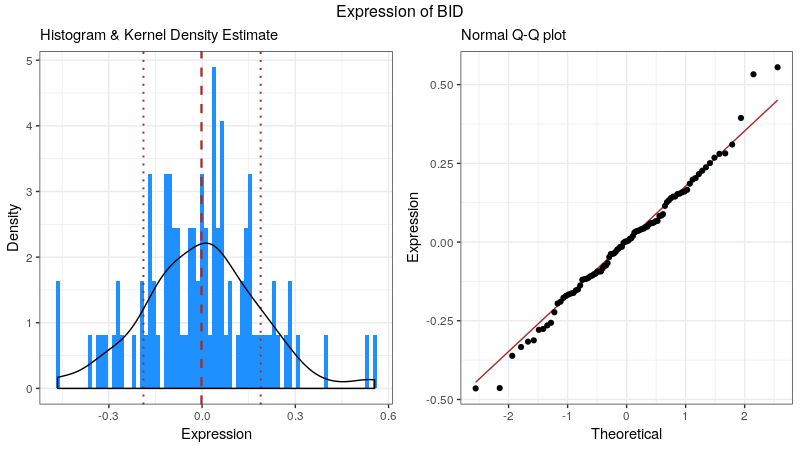
\includegraphics[height=4.8cm,width=.8\textwidth,keepaspectratio=false]{bid_expr}
  \end{subfigure}
%\end{figure}

  \begin{subfigure}{\textwidth}
%\begin{figure}[t]
    \centering
    \caption{}
% 	\caption{Scree plot and biplot of 
% the \textasciitilde800 affinities for the gene BID. In the biplot, each 
% label corresponds to an individual.}
    \labfig{pcatba}
    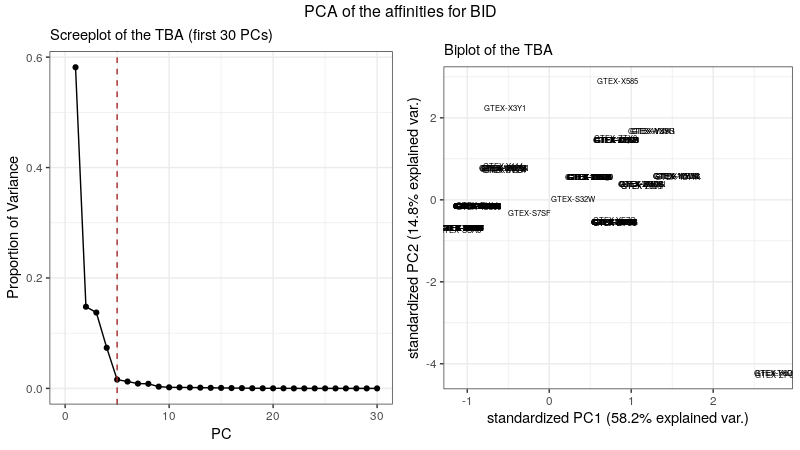
\includegraphics[height=4.8cm,width=.8\textwidth,keepaspectratio=false]{bid_tba}
  \end{subfigure}
% \end{figure}
  \caption{(a): Histogram and normal Q\babelhyphen{nobreak}Q plot of the 
expression of a randomly selected gene called BID. In the histogram, the 
brown dashed line indicates the mean, while the dotted lines indicate 
plus and minus one standard deviation. In the Q\babelhyphen{nobreak}Q 
plot, each point represents an individual. (b): Scree plot and biplot of 
the \textasciitilde800 affinities for the gene BID. In the biplot, each 
label corresponds to an individual.}
  \labfig{expl}
\end{figure}

The expression was preprocessed as recommended by the Stephen's 
Lab.\sidenote[][*7]{\url{http://stephenslab.github.io/gtex-eqtls/analysis/20170515\_RNASeq\_Analysis.html}} 
In summary, I applied a quantile normalisation to make sure that the 
distribution of our response variable was normal, and then I obtained 
the residuals of a linear model 
$Y~\sim~SEX+PEER\_FA+POPULATION+PLATFORM$, so as to disregard the 
effects of these covariates on the expression. The final result can be 
seen in \reffig{distrexpr}.

The genotypes were also obtained with a sequencing technique and were 
provided in VCF format. \sidecite[-3.2cm]{Danecek2011} I 
used a software called 
\nohyphens{VCF\textunderscore\nobreak\hspace{0pt}rider}\sidenote[][*3]{\url{https://github.com/vodkatad/vcf\_rider}} 
to compute the total binding affinity of each transcription factor for 
each regulatory region associated to a gene (the total number of 
transcription factors is about 800). \reffig{pcatba} reports the PCA of 
the TBA for the gene BID.

%==================================================================================================
\FloatBarrier
\chapter{Experiments overview}

%--------------------------------------------------------------------------------------------------
\FloatBarrier
\section{Verification of environmeint}
Because in the target implementation of a neural network, the critical element is high 
performance and small size in memory, both for the network model and for the code itself. 
Therefore, it was decided to use the C language because it provides precise control over data 
representation in memory and has minimal memory overhead for the generated code. 
During the initial phase of the experiments, a solution based on combining C with C++ 
will be used. The reason for this approach is the possibility of using design solutions and 
ready-made libraries not available in pure C, which will ensure a much shorter prototyping period.
The downside of this approach is the need to rewrite the final prototype from C ++ to pure C 
before installing it on the target platform. 
However, the experience of the research team so far shows that this approach allows for the 
fastest implementation of the project. 
The problem that resulted from this approach is the lack of direct integration of the created 
solution with the Ai Gym environment used so far, which was written in Python and requires that 
the code using it also be written in this language. 
There are three workarounds for this issue: 
\begin{enumerate}
	\item Use of a dedicated simulation environment for C / C ++.
	\item Integration between the simulation and the neural network employing a library that 
		enables the integration of C functions in Python. 
	\item Implementation of simulations and networks as separate processes together with 
		communication between them based on messages encoded in ASCII.
\end{enumerate}
The first option was immediately rejected due to delays in bringing an entirely new tool 
to the design. 
Several attempts have been made to integrate Python and C ++. This approach turned out to be 
problematic by imposing limitations on possible solutions on the C ++ side. 
An additional drawback was the low portability of the solution and a significant increase in the 
complexity of the compilation environment. 
A solution was chosen based on transferring data between two separate processes using pipes.
\begin{figure}[htb] 
	\label{fig:experiment_pipes}
	\centering
	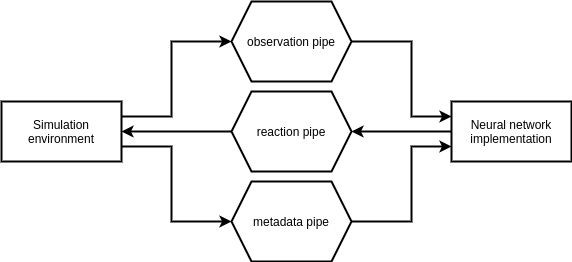
\includegraphics[width=\textwidth]{figures/experiment_pipes}
	\caption{Information flow between simulation an network.}
\end{figure}

As shown in Figure \ref{fig:experiment_pipes}, the system consists of three streams, 
observations, reactions, and metadata. 
Both the observation and reaction pipelines send single vectors separated by a space and terminated
by a line break. 
The data is then converted into the appropriate Python-side Numpy vector and C ++-side Armadillo 
matrix. 
The metadata pipeline, on the other hand, transmits additional information that is not part of 
the observation-reaction loop but is required for the correct interaction between the processes 
and for the training algorithm to be performed.
\begin{lstlisting}[language=C]
struct AiGymMetadata{
	int cycle;
	float reaward;
	int running;
	int error_code;
	string error_msg;
};
\end{lstlisting}

From the example in Listing 1, you can see five metadata elements:
\begin{enumerate}
	\item Cycle - the simulation has been divided into cycles, each of which, 
		except the zero one, is initiated by receiving a reaction and returns the 
		observation and metadata itself
	\item Reward - As part of the simulation, a reward is given for each cycle, 
		in the case of negative values it is called a penalty. 
		The exact rules for granting the awards depend on the simulation environment selected. 
	\item Simulation state - the variable takes the value of 1 when the simulation is active or 
		0 when it is stopped.
	\item Error code - if the simulation answer does not contain an error, the code is set to zero,
		otherwise the exact error code is here. In case the error code is nonzero,
		the observation pipeline is empty.  
	\item The content of the error - a detailed description of the error from the simulation, 
		allows you to send more accurate information without unnecessarily complicating the 
		metadata modelled.
\end{enumerate}

%--------------------------------------------------------------------------------------------------
\FloatBarrier
\section{Testing basic implementation of NEAT}

%--------------------------------------------------------------------------------------------------
\FloatBarrier
\section{NEAT-23, learing implementation}

%--------------------------------------------------------------------------------------------------
\FloatBarrier
\section{NEAT-23, execution implementation}

%--------------------------------------------------------------------------------------------------
\FloatBarrier
\section{On device}

\section{Discussion}
\labsec{discussion}

Instead of finding a better model, in this project I tried to find 
better predictors. Using the affinities instead of the genotypes has 
several advantages:

\begin{itemize}
  \item The model is more interpretable;
  \item The number of predictors decreases;
  \item The predictive power is higher;
\end{itemize}

Upon doing some biochemical considerations, it is possible to find even 
better predictors, although they violate the constraint of using only 
the DNA sequence to predict gene expression.

There are many ways to continue this work. One would be to construct an 
ensemble model that chooses, for each gene, the model that achieved the 
best prediction on a training set.

Another possibility is that of exploiting further the interpretability 
of this model, and use the trees produced by BART to make inferences 
about the regulatory network among genes.

Finally, one of the biggest limitations of these kind of models is that 
they consider each gene as independent of all the others. One possible 
way to use the information hidden among other genes is what I call the 
\enquote{bagging of the genes,} where the prediction for a new gene is 
given by the average of the prediction of a number of other models 
trained on different genes.

If we were able to accurately predict gene expression, the benefit would 
be twofold: first, it would be possible to predict which individuals are 
at risk of developing a disease, and consequently to prevent it; 
secondly, the biological mechanisms through which the illnesses arise 
would be elucidated, potentially leading to the discovery of new 
therapeutic targets. In conclusion, I hope that this project will give a 
contribution, albeit very small, in understanding the relationships 
between genome, expression and diseases.


\defbibnote{bibnote}{Here are the references in citation order.\par\bigskip} % Prepend this text to the bibliography
\renewcommand*{\bibfont}{\small}
\printbibliography[title=Bibliography]% , prenote=bibnote]

\end{document}
